\chapter{Implementation: Version Control, CI, and Coding Standards}
\label{ch:implementation}

\begin{quote}
\emph{``Weeks of coding can save you hours of planning.''} But disciplined implementation---branching, reviewing, and integrating continuously---turns that joke into sustainable throughput.
\end{quote}

\noindent\fbox{\parbox{\dimexpr\linewidth-2\fboxsep-2\fboxrule}{%
\textbf{From zero: no prior Git/CI experience assumed.} We define \emph{repository}, \emph{branch}, \emph{pull request}, \emph{continuous integration}, and \emph{coding standard} from first principles---intuition and diagrams before commands. We assume only Ch.~3--4 (design and sprints): code now realises the blueprint in measured increments.}}

\vspace{0.4em}

\section*{Learning Outcomes}
After this chapter you will be able to:
\begin{enumerate}[label=(L\arabic*)]
    \item use Git effectively: branching, merging, and pull-request workflows with code review;
    \item design a CI pipeline that builds, tests, and lints on every push and blocks broken merges;
    \item apply coding standards, documentation, and refactoring to keep a shared codebase maintainable;
    \item manage dependencies and configuration across environments without ``works on my machine'';
    \item resolve merge conflicts and recover from common Git failures calmly.
\end{enumerate}

% ============================================================
\section{Version Control with Git: From Snapshots to Collaboration}
\label{sec:vcs}

\textbf{Intuition.} Without version control, collaboration is emailing \texttt{project\_final\_v3\_REAL.zip}. Git replaces that with a \emph{directed acyclic graph} (DAG) of snapshots: each commit points to its parent(s); branches are movable labels; merges create join commits.

\begin{definition}[Repository, Commit, Branch]
A \emph{repository} is the complete history. A \emph{commit} is an immutable snapshot plus metadata (author, message, parent). A \emph{branch} is a pointer to a commit that advances with new commits.
\end{definition}

\begin{figure}[h]
\centering
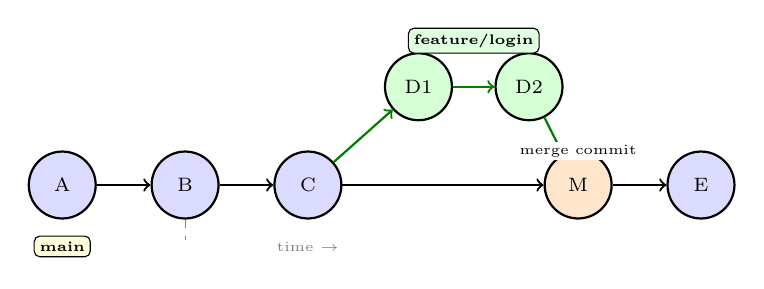
\begin{tikzpicture}[scale=0.78, every node/.style={font=\scriptsize},
  commit/.style={draw,thick,circle,minimum size=0.85cm,align=center,fill=blue!14},
  merge/.style={draw,thick,circle,minimum size=0.85cm,align=center,fill=orange!20},
  branchlab/.style={font=\tiny\bfseries,fill=yellow!15,draw,rounded corners=2pt,inner sep=2pt}]
  % main line
  \node[commit] (a) at (0,0) {A};
  \node[commit] (b) at (2.0,0) {B};
  \node[commit] (c) at (4.0,0) {C};
  \node[merge]  (m) at (8.4,0) {M};
  \node[commit] (e) at (10.4,0) {E};
  \draw[->,thick] (a) -- (b); \draw[->,thick] (b) -- (c);
  \draw[->,thick] (c) -- (m); \draw[->,thick] (m) -- (e);
  % feature branch
  \node[commit,fill=green!16] (d1) at (5.8,1.6) {D1};
  \node[commit,fill=green!16] (d2) at (7.6,1.6) {D2};
  \draw[->,thick,green!50!black] (c) -- (d1); \draw[->,thick,green!50!black] (d1) -- (d2);
  \draw[->,thick,green!50!black] (d2) -- (m);
  % labels
  \node[branchlab] at (0,-1.0) {main};
  \node[branchlab,fill=green!12] at (6.7,2.35) {feature/login};
  \node[font=\tiny,gray] at (4.0,-1.0) {time $\to$};
  \node[font=\tiny,fill=white,inner sep=1pt] at (8.4,0.55) {merge commit};
  \draw[dashed,gray] (b) -- (b |- 0,-0.9);
\end{tikzpicture}
\caption{Git DAG: main advances A$\to$B$\to$C; feature branches at C, adds D1--D2, merges back as M. Colours distinguish main (blue) from feature (green) and merge (orange). Conflicts are resolved at M, not by overwriting.}
\label{fig:git-dag}
\end{figure}

\textbf{Branching for capstone.} Keep \texttt{main} always green (CI passing, deployable). Work on short-lived feature branches (\texttt{feature/}, \texttt{fix/}) cut from \texttt{main}; open a \emph{pull request} (PR) when ready; require one peer review and green CI before merge. This is \emph{GitHub Flow}---simple enough for a 4-person team. GitFlow (develop/release/hotfix branches) is overkill unless you manage parallel releases.

PR hygiene: small diffs ($<400$ lines), descriptive title, checklist (tests added, docs updated, linked issue). Review for correctness, design fit, and standards---not style bikeshedding that a linter could catch.

\begin{figure}[h]
\centering
\begin{tikzpicture}[scale=0.78, every node/.style={font=\scriptsize},
  box/.style={draw,thick,rounded corners=3pt,minimum width=2.3cm,minimum height=0.85cm,align=center},
  arr/.style={-{Stealth[length=2.6mm]},thick,blue!60!black}]
  \node[box,fill=blue!14] (branch) at (0,0) {Create branch\\{\tiny\texttt{git switch -c feat/x}}};
  \node[box,fill=green!14] (commit) at (3.8,0) {Commit locally\\{\tiny atomic + message}};
  \node[box,fill=orange!16] (push) at (7.6,0) {Push + open PR\\{\tiny CI runs}};
  \node[box,fill=violet!14] (review) at (7.6,-1.7) {Review\\{\tiny 1 approval}};
  \node[box,fill=teal!14] (merge) at (3.8,-1.7) {Squash \& merge\\{\tiny to main}};
  \node[box,fill=gray!12] (pull) at (0,-1.7) {Pull main\\{\tiny keep local fresh}};
  \draw[arr] (branch) -- (commit);
  \draw[arr] (commit) -- (push);
  \draw[arr] (push) -- (review);
  \draw[arr] (review) -- (merge);
  \draw[arr] (merge) -- (pull);
  \draw[arr,dashed,red!60!black] (review) -- ++(-2.0,0) |- (commit) node[pos=0.25,left,font=\tiny,fill=white] {changes requested};
  \node[font=\tiny,gray,align=center] at (3.8,-2.6) {Every transition is a quality gate; blocked PR = unmerged risk isolated on branch};
\end{tikzpicture}
\caption{Pull-request workflow as a state machine. Dashed feedback is normal; the merge gate protects main from red builds and unreviewed code.}
\label{fig:pr-workflow}
\end{figure}

Merge conflicts occur when two branches edit the same lines. Git marks \texttt{<<<<<<< HEAD} regions; edit to combine intent (not just pick one side), test, then commit the resolution. Prevent conflicts by pulling \texttt{main} daily, splitting work by feature not by file, and communicating who owns which module this sprint.

% ============================================================
\section{Continuous Integration: Build, Test, Lint on Every Push}
\label{sec:ci}

Manual testing before submission is a gamble. \emph{Continuous Integration} (CI) runs an automated pipeline on every push: install dependencies, lint, build, run tests, and report status on the PR.

\begin{definition}[CI Pipeline]
An automated sequence triggered by a push or PR that reproducibly builds the system and verifies quality gates. A red pipeline blocks merge; a green pipeline is necessary but not sufficient for approval.
\end{definition}

A minimal capstone pipeline (GitHub Actions / GitLab CI) has four jobs: \texttt{lint} (ESLint/Flake8/Checkstyle), \texttt{test} (unit + integration), \texttt{build} (compile/bundle), and \texttt{security} (dependency audit). Cache dependencies to keep runs under 3~minutes---slow CI is ignored CI.

\begin{lstlisting}[language=Python,caption={Minimal CI config sketch (GitHub Actions): lint, test, and block on failure.},label={lst:ci-config}]
# .github/workflows/ci.yml
name: CI
on: [push, pull_request]
jobs:
  ci:
    runs-on: ubuntu-latest
    steps:
      - uses: actions/checkout@v4
      - uses: actions/setup-python@v5
        with: { python-version: '3.11' }
      - run: pip install -r requirements.txt
      - run: ruff check .          # lint -- must pass
      - run: pytest --cov --cov-fail-under=70  # 70% floor
      - run: python -m build       # ensure it bundles
\end{lstlisting}

Enforce branch protection: \texttt{main} requires green CI and one approval. Add a badge to \texttt{README.md}; its colour is a team health signal. Deployment (CD) can auto-deploy \texttt{main} to a staging environment, but keep production deploys manual and tagged (\texttt{v0.3.0}) during capstone.

{\sloppy Secrets (API keys, DB passwords) never enter Git. Use environment variables or a vault; commit a \texttt{.env.example} with dummy values. History rewrites (\texttt{filter-branch}) are painful---exclusion is cheaper than cleanup.\par}

% ============================================================
\section{Coding Standards, Documentation, and Sustainable Pace}
\label{sec:standards}

Standards make code readable by strangers---including future you. Adopt an existing guide (PEP~8 for Python, Google Java Style, Airbnb JS) and enforce it with a formatter (\texttt{black}, \texttt{prettier}, \texttt{google-java-format}) and linter so reviews discuss design, not spacing.

Key practices:
\begin{itemize}
    \item \textbf{Naming:} intent-revealing (\texttt{calculateETA()} not \texttt{doCalc()}), consistent casing, and no abbreviations that need a glossary.
    \item \textbf{Functions:} small (20--30 lines), single responsibility, early returns; cyclomatic complexity $<10$.
    \item \textbf{Comments:} explain \emph{why}, not \emph{what}; docstrings for public APIs with params/returns and one example.
    \item \textbf{Refactoring:} rename, extract method, and isolate side effects continuously; never mix feature and refactor in one PR.
\end{itemize}

\begin{figure}[h]
\centering
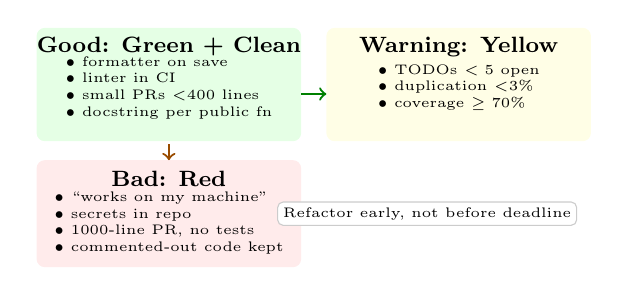
\begin{tikzpicture}[scale=0.80, every node/.style={font=\scriptsize}]
  \fill[green!10,rounded corners=3pt] (0,0) rectangle (4.2,1.8);
  \fill[yellow!10,rounded corners=3pt] (4.6,0) rectangle (8.8,1.8);
  \fill[red!8,rounded corners=3pt] (0,-2.0) rectangle (4.2,-0.3);
  \node[font=\footnotesize\bfseries] at (2.1,1.50) {Good: Green + Clean};
  \node[font=\tiny,align=left] at (2.1,0.85) {$\bullet$ formatter on save\\$\bullet$ linter in CI\\$\bullet$ small PRs $<$400 lines\\$\bullet$ docstring per public fn};
  \node[font=\footnotesize\bfseries] at (6.7,1.50) {Warning: Yellow};
  \node[font=\tiny,align=left] at (6.7,0.85) {$\bullet$ TODOs $<5$ open\\$\bullet$ duplication $<$3\%\\$\bullet$ coverage $\ge 70$\%};
  \node[font=\footnotesize\bfseries] at (2.1,-0.60) {Bad: Red};
  \node[font=\tiny,align=left] at (2.1,-1.30) {$\bullet$ ``works on my machine''\\$\bullet$ secrets in repo\\$\bullet$ 1000-line PR, no tests\\$\bullet$ commented-out code kept};
  \draw[->,thick,green!50!black] (4.2,0.75) -- (4.6,0.75);
  \draw[->,thick,orange!60!black] (2.1,-0.05) -- (2.1,-0.30);
  \node[font=\tiny,align=center,fill=white,draw=gray!40,rounded corners=2pt,inner sep=2pt] at (6.2,-1.15) {Refactor early, not before deadline};
\end{tikzpicture}
\caption{Code-health traffic light: green practices let reviews focus on design; yellow signals need attention; red must block merge via CI and human gates.}
\label{fig:code-health}
\end{figure}

Manage dependencies with a lockfile
(\texttt{requirements.txt}/\texttt{poetry.lock},
\texttt{package-lock.json}) and pin versions. Use the
\texttt{.env} file for configuration per environment
(dev/staging/prod) and document every variable in
\texttt{.env.example}. Containerise
(\texttt{Dockerfile} + \texttt{docker-compose.yml})
when the team hits ``works on my machine''---the image
\emph{is} the environment.

% ============================================================
\section{Dependencies, Configuration, and Recovery}
\label{sec:deps-recovery}

Real projects break on ``works on my machine'' because each laptop has different Node/Python/DB versions. Two fixes repeat.

\paragraph{Lockfiles and reproducible builds.} A manifest (\texttt{requirements.in}, \texttt{package.json}) declares \emph{ranges}; the lockfile pins \emph{exact} resolved versions. Commit both. CI installs from the lockfile, not the manifest, so every runner resolves identically. Run \texttt{pip-audit} or \texttt{npm audit} weekly and update via a dedicated PR---never bundle dependency bumps with feature code.

\paragraph{Configuration as environment.} Twelve-factor principle: config varies per deploy, code does not. Never branch on \texttt{if prod:}. Instead read \texttt{DATABASE\_URL}, \texttt{STRIPE\_KEY}, \texttt{LOG\_LEVEL} from the environment. Provide \texttt{.env.example} with safe defaults and document each variable's purpose and required format in \texttt{README.md}.

\paragraph{Common Git recoveries.} Keep these in your team wiki:
\begin{itemize}
    \item \textbf{Wrong commit message:} \texttt{git commit --amend} (before push) or revert.
    \item \textbf{Committed secret:} revoke credential immediately, then \texttt{git revert}; history rewrite is rarely worth the disruption during a semester---rotation is the real fix.
    \item \textbf{Detached HEAD / lost commit:} \texttt{git reflog} shows every HEAD move; \texttt{git cherry-pick} the hash back.
    \item {\sloppy \textbf{Merge vs.\ rebase on shared branches:} merge preserves history and is safe for shared \texttt{main}; rebase rewrites and is only for private feature branches before PR. Agree per team and enforce via \texttt{CONTRIBUTING.md}.\par}
\end{itemize}

\begin{example}[Docker as the equaliser]
A one-service \texttt{docker-compose.yml} that starts app + Postgres + seed data removes ``install Postgres 15.2 and create role X'' from onboarding. New teammate runs \texttt{docker compose up --build} and is running in 3~minutes. CI uses the same image, so environment drift vanishes as a bug category.
\end{example}

\begin{remark}[Checklist before merge]
Before you click ``Merge'' verify: CI green, one approval, no TODO without issue link, \texttt{.env.example} updated, and linked issue moved to Done. A 30-second scan here saves a 30-minute revert later. Keep PRs under 400 lines; large PRs are rarely reviewed well and hide defects. Tag releases (\texttt{v0.4.0}) so demo and report cite the same immutable artefact.
\end{remark}

\begin{example}[Commit message that helps]
\texttt{feat(auth): add JWT refresh with 7-day expiry} --- prefix (\texttt{feat}/\texttt{fix}/\texttt{docs}), scope (\texttt{auth}), imperative description, and body that cites the issue and risk. A year later, \texttt{git log --grep=auth} finds every auth change; \texttt{git blame} explains why a line exists. Good messages are documentation that never drifts from code.
\end{example}

% ============================================================
\section{Exercises}
\label{sec:ch05-exercises}
\begin{enumerate}[label=E5.\arabic*, leftmargin=*, itemsep=0.6em]
    \item \textbf{Git DAG reasoning.} Starting from Fig.~\ref{fig:git-dag}, developer X merges \texttt{feature/login} into \texttt{main} as M, then Y pushes commit F to \texttt{main} before X pulls. Draw the resulting DAG, explain why a fast-forward is impossible, and give the two commands to reconcile (merge vs.\ rebase) with trade-offs for a shared branch.
    \item \textbf{Branch protection design.} Your 4-person team uses GitHub Flow. Write branch-protection rules for \texttt{main} (required checks, approvals, stale-review dismissal) and justify each. What breaks if you allow direct pushes to \texttt{main} even with CI?
    \item \textbf{CI pipeline critique.} A teammate proposes CI that runs only \texttt{pytest} (no lint, no build, no coverage floor). List three defects this misses, add them as pipeline jobs with failure conditions, and estimate the cost of catching each defect in CI versus in sprint review versus after release.
    \item \textbf{Refactor PR.} A file \texttt{report.py} (320 lines) generates PDFs, queries the DB, and emails reports---one PR adds a new report type inline. Apply SRP to split it, draft the new module boundaries, and rewrite the PR as two sequential PRs (refactor then feature) with test plans for each.
    \item \textbf{Secrets and environments.} Your repo accidentally committed \texttt{.env} containing a Stripe test key. List immediate remediation steps (revoke, purge, prevent) and design a configuration scheme (\texttt{.env.example}, env vars, CI secrets) so staging and production use different keys without branching.
\end{enumerate}
% End of Chapter 5
